\documentclass[12pt]{article}
\usepackage{amsmath,latexsym,amsfonts,amssymb,graphicx,amsthm,epsfig,enumerate}
\usepackage{tikz,verbatim} % adds charting fuctions

\linespread{1.2}

%\pagestyle{empty}

\begin{document}
		\title{Title} %add title here
		\author{Name} %add names here
		% add other necessary information here
		
		\maketitle
		\thispagestyle{empty}
		\newpage
		
		\section{Introduction}
		
		\subsection{Architecture}
		\begin{figure}[!h]
			\centering
		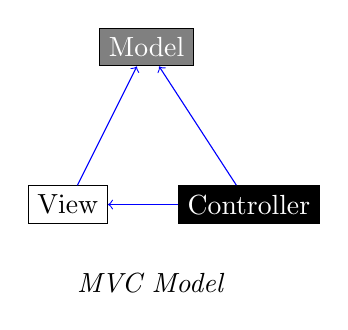
\begin{tikzpicture}
		% MVC Architecture
		\node[draw] (View) at (0,0) {View};
		\node[draw,fill=black,text=white] (Controller) at (2.3,0) {Controller};
		\node[draw,fill=gray,text=white] (Model) at (1,2) {Model};

		\draw[->,draw=blue] (View) to (Model);
		\draw[->,draw=blue] (Controller) to (View);
		\draw[->,draw=blue] (Controller) to (Model);
		\node at (1.0, -1.0) {\textit{ MVC Model}};
		
		\end{tikzpicture}
		\end{figure}
		This software uses MVC architecture in its design. 
		\subsection{Technologies}
		\begin{itemize}
		\item Java:  An object oriented programming language 
		\item Eclipse: 
		\item Java Swing: A java toolkit designed to aid programmers in the creation of gui applications. This widget toolkit allows the programmer quick access to various predefined graphical objects, allowing the easy creation of a graphical interface.
		
		\end{itemize}
		\section{Modular Decomposition}
		% 4.1Description of the classes and modules and why they were used
		\section{Module Guide}
		%4.2 For each module, a description of the interface and behaviors of each method
		\section{Traceability}
		% 4.5 A Description of each class
		% Tablular Expressions
		\begin{tabular}{|c|c|c|}
			Thing & Other Thing & Output \\
			\hline \\
			
		\end{tabular}
		\section{Uses Relation}
		% A diagram and brief description describing why how the stufff interacts
		
		\section{Testing}
		% A section on the testing of the software
		%Behavoir Table
		\begin{tabular}{|c|c|c|}
			What you tested & What it did & Comments on that \\
			\hline \\
			
		\end{tabular}
			
		\section{Discussion}
		%4.6 Internal review/ evaluation of design
		\subsection{Anticipated Changes}
		% what was designed in anticipation of changes
		
	
\end{document}